\documentclass[1p]{elsarticle_modified}
%\bibliographystyle{elsarticle-num}

%\usepackage[colorlinks]{hyperref}
%\usepackage{abbrmath_seonhwa} %\Abb, \Ascr, \Acal ,\Abf, \Afrak
\usepackage{amsfonts}
\usepackage{amssymb}
\usepackage{amsmath}
\usepackage{amsthm}
\usepackage{scalefnt}
\usepackage{amsbsy}
\usepackage{kotex}
\usepackage{caption}
\usepackage{subfig}
\usepackage{color}
\usepackage{graphicx}
\usepackage{xcolor} %% white, black, red, green, blue, cyan, magenta, yellow
\usepackage{float}
\usepackage{setspace}
\usepackage{hyperref}

\usepackage{tikz}
\usetikzlibrary{arrows}

\usepackage{multirow}
\usepackage{array} % fixed length table
\usepackage{hhline}

%%%%%%%%%%%%%%%%%%%%%
\makeatletter
\renewcommand*\env@matrix[1][\arraystretch]{%
	\edef\arraystretch{#1}%
	\hskip -\arraycolsep
	\let\@ifnextchar\new@ifnextchar
	\array{*\c@MaxMatrixCols c}}
\makeatother %https://tex.stackexchange.com/questions/14071/how-can-i-increase-the-line-spacing-in-a-matrix
%%%%%%%%%%%%%%%

\usepackage[normalem]{ulem}

\newcommand{\msout}[1]{\ifmmode\text{\sout{\ensuremath{#1}}}\else\sout{#1}\fi}
%SOURCE: \msout is \stkout macro in https://tex.stackexchange.com/questions/20609/strikeout-in-math-mode

\newcommand{\cancel}[1]{
	\ifmmode
	{\color{red}\msout{#1}}
	\else
	{\color{red}\sout{#1}}
	\fi
}

\newcommand{\add}[1]{
	{\color{blue}\uwave{#1}}
}

\newcommand{\replace}[2]{
	\ifmmode
	{\color{red}\msout{#1}}{\color{blue}\uwave{#2}}
	\else
	{\color{red}\sout{#1}}{\color{blue}\uwave{#2}}
	\fi
}

\newcommand{\Sol}{\mathcal{S}} %segment
\newcommand{\D}{D} %diagram
\newcommand{\A}{\mathcal{A}} %arc


%%%%%%%%%%%%%%%%%%%%%%%%%%%%%5 test

\def\sl{\operatorname{\textup{SL}}(2,\Cbb)}
\def\psl{\operatorname{\textup{PSL}}(2,\Cbb)}
\def\quan{\mkern 1mu \triangleright \mkern 1mu}

\theoremstyle{definition}
\newtheorem{thm}{Theorem}[section]
\newtheorem{prop}[thm]{Proposition}
\newtheorem{lem}[thm]{Lemma}
\newtheorem{ques}[thm]{Question}
\newtheorem{cor}[thm]{Corollary}
\newtheorem{defn}[thm]{Definition}
\newtheorem{exam}[thm]{Example}
\newtheorem{rmk}[thm]{Remark}
\newtheorem{alg}[thm]{Algorithm}

\newcommand{\I}{\sqrt{-1}}
\begin{document}

%\begin{frontmatter}
%
%\title{Boundary parabolic representations of knots up to 8 crossings}
%
%%% Group authors per affiliation:
%\author{Yunhi Cho} 
%\address{Department of Mathematics, University of Seoul, Seoul, Korea}
%\ead{yhcho@uos.ac.kr}
%
%
%\author{Seonhwa Kim} %\fnref{s_kim}}
%\address{Center for Geometry and Physics, Institute for Basic Science, Pohang, 37673, Korea}
%\ead{ryeona17@ibs.re.kr}
%
%\author{Hyuk Kim}
%\address{Department of Mathematical Sciences, Seoul National University, Seoul 08826, Korea}
%\ead{hyukkim@snu.ac.kr}
%
%\author{Seokbeom Yoon}
%\address{Department of Mathematical Sciences, Seoul National University, Seoul, 08826,  Korea}
%\ead{sbyoon15@snu.ac.kr}
%
%\begin{abstract}
%We find all boundary parabolic representation of knots up to 8 crossings.
%
%\end{abstract}
%\begin{keyword}
%    \MSC[2010] 57M25 
%\end{keyword}
%
%\end{frontmatter}

%\linenumbers
%\tableofcontents
%
\newcommand\colored[1]{\textcolor{white}{\rule[-0.35ex]{0.8em}{1.4ex}}\kern-0.8em\color{red} #1}%
%\newcommand\colored[1]{\textcolor{white}{ #1}\kern-2.17ex	\textcolor{white}{ #1}\kern-1.81ex	\textcolor{white}{ #1}\kern-2.15ex\color{red}#1	}

{\Large $\underline{12a_{0374}~(K12a_{0374})}$}

\setlength{\tabcolsep}{10pt}
\renewcommand{\arraystretch}{1.6}
\vspace{1cm}\begin{tabular}{m{100pt}>{\centering\arraybackslash}m{274pt}}
\multirow{5}{120pt}{
	\centering
	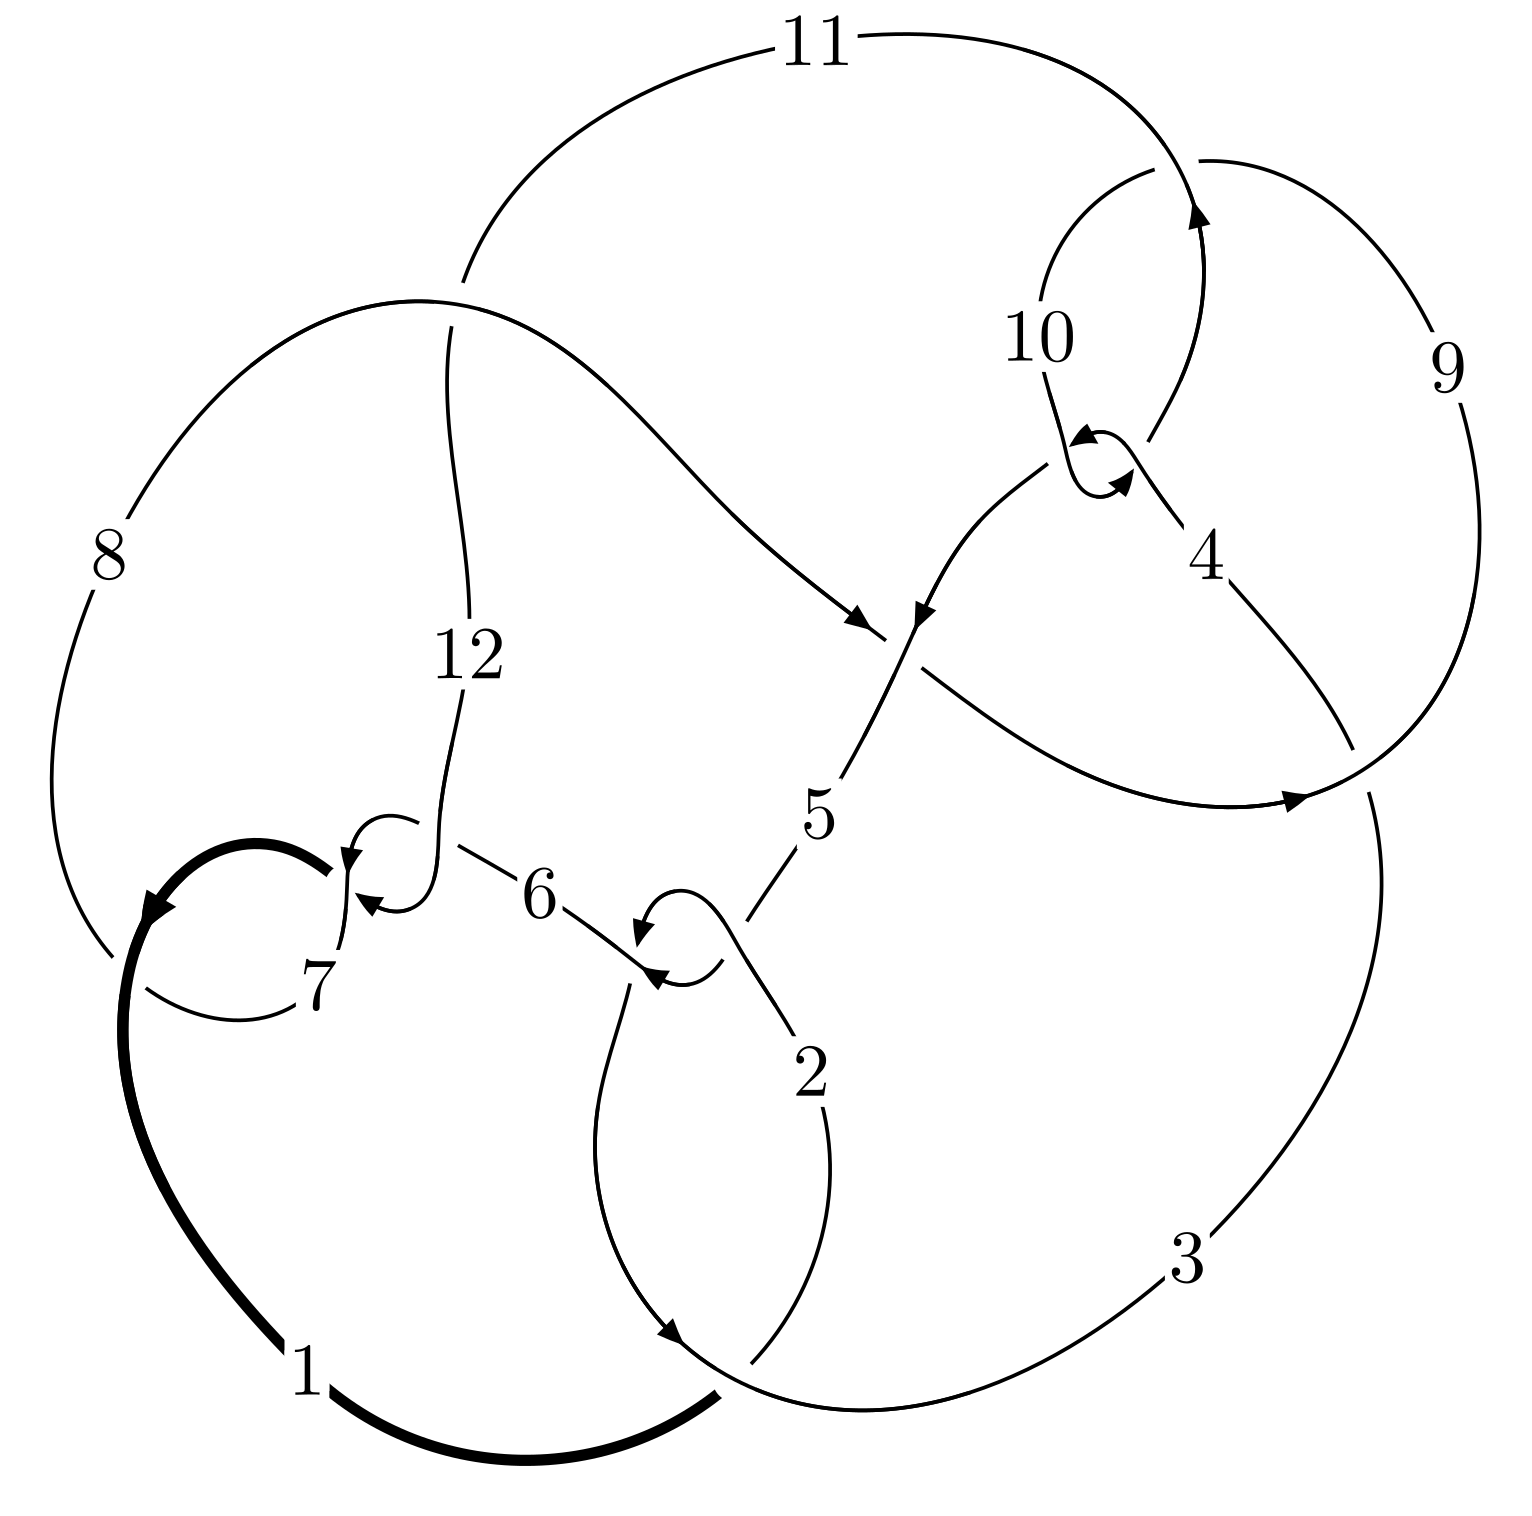
\includegraphics[width=112pt]{../../../GIT/diagram.site/Diagrams/png/1175_12a_0374.png}\\
\ \ \ A knot diagram\footnotemark}&
\allowdisplaybreaks
\textbf{Linearized knot diagam} \\
\cline{2-2}
 &
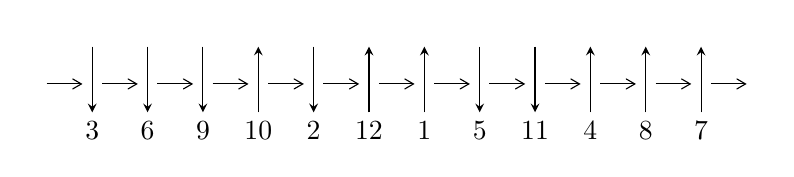
\begin{tikzpicture}[x=20pt, y=17pt]
	% nodes
	\node (C0) at (0, 0) {};
	\node (C1) at (1, 0) {};
	\node (C1U) at (1, +1) {};
	\node (C1D) at (1, -1) {3};

	\node (C2) at (2, 0) {};
	\node (C2U) at (2, +1) {};
	\node (C2D) at (2, -1) {6};

	\node (C3) at (3, 0) {};
	\node (C3U) at (3, +1) {};
	\node (C3D) at (3, -1) {9};

	\node (C4) at (4, 0) {};
	\node (C4U) at (4, +1) {};
	\node (C4D) at (4, -1) {10};

	\node (C5) at (5, 0) {};
	\node (C5U) at (5, +1) {};
	\node (C5D) at (5, -1) {2};

	\node (C6) at (6, 0) {};
	\node (C6U) at (6, +1) {};
	\node (C6D) at (6, -1) {12};

	\node (C7) at (7, 0) {};
	\node (C7U) at (7, +1) {};
	\node (C7D) at (7, -1) {1};

	\node (C8) at (8, 0) {};
	\node (C8U) at (8, +1) {};
	\node (C8D) at (8, -1) {5};

	\node (C9) at (9, 0) {};
	\node (C9U) at (9, +1) {};
	\node (C9D) at (9, -1) {11};

	\node (C10) at (10, 0) {};
	\node (C10U) at (10, +1) {};
	\node (C10D) at (10, -1) {4};

	\node (C11) at (11, 0) {};
	\node (C11U) at (11, +1) {};
	\node (C11D) at (11, -1) {8};

	\node (C12) at (12, 0) {};
	\node (C12U) at (12, +1) {};
	\node (C12D) at (12, -1) {7};
	\node (C13) at (13, 0) {};

	% arrows
	\draw[->,>={angle 60}]
	(C0) edge (C1) (C1) edge (C2) (C2) edge (C3) (C3) edge (C4) (C4) edge (C5) (C5) edge (C6) (C6) edge (C7) (C7) edge (C8) (C8) edge (C9) (C9) edge (C10) (C10) edge (C11) (C11) edge (C12) (C12) edge (C13) ;	\draw[->,>=stealth]
	(C1U) edge (C1D) (C2U) edge (C2D) (C3U) edge (C3D) (C4D) edge (C4U) (C5U) edge (C5D) (C6D) edge (C6U) (C7D) edge (C7U) (C8U) edge (C8D) (C9U) edge (C9D) (C10D) edge (C10U) (C11D) edge (C11U) (C12D) edge (C12U) ;
	\end{tikzpicture} \\
\hhline{~~} \\& 
\textbf{Solving Sequence} \\ \cline{2-2} 
 &
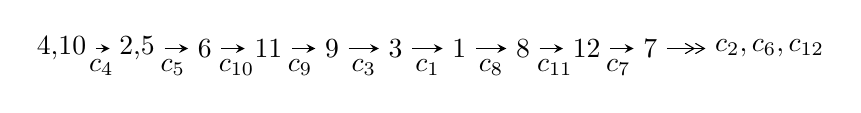
\begin{tikzpicture}[x=23pt, y=7pt]
	% node
	\node (A0) at (-1/8, 0) {4,10};
	\node (A1) at (17/16, 0) {2,5};
	\node (A2) at (17/8, 0) {6};
	\node (A3) at (25/8, 0) {11};
	\node (A4) at (33/8, 0) {9};
	\node (A5) at (41/8, 0) {3};
	\node (A6) at (49/8, 0) {1};
	\node (A7) at (57/8, 0) {8};
	\node (A8) at (65/8, 0) {12};
	\node (A9) at (73/8, 0) {7};
	\node (C1) at (1/2, -1) {$c_{4}$};
	\node (C2) at (13/8, -1) {$c_{5}$};
	\node (C3) at (21/8, -1) {$c_{10}$};
	\node (C4) at (29/8, -1) {$c_{9}$};
	\node (C5) at (37/8, -1) {$c_{3}$};
	\node (C6) at (45/8, -1) {$c_{1}$};
	\node (C7) at (53/8, -1) {$c_{8}$};
	\node (C8) at (61/8, -1) {$c_{11}$};
	\node (C9) at (69/8, -1) {$c_{7}$};
	\node (A10) at (11, 0) {$c_{2},c_{6},c_{12}$};

	% edge
	\draw[->,>=stealth]	
	(A0) edge (A1) (A1) edge (A2) (A2) edge (A3) (A3) edge (A4) (A4) edge (A5) (A5) edge (A6) (A6) edge (A7) (A7) edge (A8) (A8) edge (A9) ;
	\draw[->>,>={angle 60}]	
	(A9) edge (A10);
\end{tikzpicture} \\ 

\end{tabular} \\

\footnotetext{
The image of knot diagram is generated by the software ``\textbf{Draw programme}" developed by Andrew Bartholomew(\url{http://www.layer8.co.uk/maths/draw/index.htm\#Running-draw}), where we modified some parts for our purpose(\url{https://github.com/CATsTAILs/LinksPainter}).
}\phantom \\ \newline 
\centering \textbf{Ideals for irreducible components\footnotemark of $X_{\text{par}}$} 
 
\begin{align*}
I^u_{1}&=\langle 
3 u^{69}+4 u^{68}+\cdots+4 b-4,\;-2 u^{70}- u^{69}+\cdots+4 a-2,\;u^{71}+2 u^{70}+\cdots-4 u-2\rangle \\
I^u_{2}&=\langle 
-20 u^3 a^2-83 u^3 a+\cdots-210 a+142,\\
\phantom{I^u_{2}}&\phantom{= \langle  }-2 u^3 a^2+u^3 a+a^3-2 a^2 u-3 u^2 a- u^3-2 a^2- a u-2 u^2+2 a- u+1,\;u^4+u^2+u+1\rangle \\
I^u_{3}&=\langle 
- u^3+b- u+1,\;- u^3+2 u^2+2 a+4,\;u^4+2 u^2+2\rangle \\
I^u_{4}&=\langle 
-5 u^5 a^2+15 u^5 a+\cdots-30 a+24,\;-2 u^4 a^2- u^4 a-2 a^2 u^2+3 u^3 a- u^4+a^3+u^3+2 a u- u^2+1,\\
\phantom{I^u_{4}}&\phantom{= \langle  }u^6- u^5+2 u^4-2 u^3+2 u^2-2 u+1\rangle \\
\\
I^v_{1}&=\langle 
a,\;b+1,\;v-1\rangle \\
\end{align*}
\raggedright * 5 irreducible components of $\dim_{\mathbb{C}}=0$, with total 106 representations.\\
\footnotetext{All coefficients of polynomials are rational numbers. But the coefficients are sometimes approximated in decimal forms when there is not enough margin.}
\newpage
\renewcommand{\arraystretch}{1}
\centering \section*{I. $I^u_{1}= \langle 3 u^{69}+4 u^{68}+\cdots+4 b-4,\;-2 u^{70}- u^{69}+\cdots+4 a-2,\;u^{71}+2 u^{70}+\cdots-4 u-2 \rangle$}
\flushleft \textbf{(i) Arc colorings}\\
\begin{tabular}{m{7pt} m{180pt} m{7pt} m{180pt} }
\flushright $a_{4}=$&$\begin{pmatrix}1\\0\end{pmatrix}$ \\
\flushright $a_{10}=$&$\begin{pmatrix}0\\u\end{pmatrix}$ \\
\flushright $a_{2}=$&$\begin{pmatrix}\frac{1}{2} u^{70}+\frac{1}{4} u^{69}+\cdots-\frac{3}{2} u+\frac{1}{2}\\-\frac{3}{4} u^{69}- u^{68}+\cdots+\frac{1}{2} u+1\end{pmatrix}$ \\
\flushright $a_{5}=$&$\begin{pmatrix}1\\- u^2\end{pmatrix}$ \\
\flushright $a_{6}=$&$\begin{pmatrix}-\frac{1}{2} u^{70}- u^{69}+\cdots+u+\frac{3}{2}\\- u^{70}- u^{69}+\cdots+\frac{3}{2} u+1\end{pmatrix}$ \\
\flushright $a_{11}=$&$\begin{pmatrix}u\\u\end{pmatrix}$ \\
\flushright $a_{9}=$&$\begin{pmatrix}u^3\\u^3+u\end{pmatrix}$ \\
\flushright $a_{3}=$&$\begin{pmatrix}- u^6- u^4+1\\- u^6-2 u^4- u^2\end{pmatrix}$ \\
\flushright $a_{1}=$&$\begin{pmatrix}\frac{1}{2} u^{70}+\frac{17}{2} u^{68}+\cdots-2 u-\frac{1}{2}\\- u^{69}- u^{68}+\cdots+\frac{1}{2} u+1\end{pmatrix}$ \\
\flushright $a_{8}=$&$\begin{pmatrix}u^5+2 u^3+u\\- u^7- u^5+u\end{pmatrix}$ \\
\flushright $a_{12}=$&$\begin{pmatrix}u^{13}+4 u^{11}+7 u^9+6 u^7+2 u^5+u\\- u^{15}-3 u^{13}-4 u^{11}- u^9+2 u^7+2 u^5+u\end{pmatrix}$ \\
\flushright $a_{7}=$&$\begin{pmatrix}\frac{1}{4} u^{56}+\frac{13}{4} u^{54}+\cdots+\frac{1}{2} u+\frac{1}{2}\\\frac{1}{4} u^{56}+\frac{7}{2} u^{54}+\cdots-\frac{1}{2} u^2+u\end{pmatrix}$\\&\end{tabular}
\flushleft \textbf{(ii) Obstruction class $= -1$}\\~\\
\flushleft \textbf{(iii) Cusp Shapes $= -2 u^{70}-4 u^{69}+\cdots+4 u^2-2 u$}\\~\\
\newpage\renewcommand{\arraystretch}{1}
\flushleft \textbf{(iv) u-Polynomials at the component}\newline \\
\begin{tabular}{m{50pt}|m{274pt}}
Crossings & \hspace{64pt}u-Polynomials at each crossing \\
\hline $$\begin{aligned}c_{1}\end{aligned}$$&$\begin{aligned}
&u^{71}+34 u^{70}+\cdots+9 u+1
\end{aligned}$\\
\hline $$\begin{aligned}c_{2},c_{5}\end{aligned}$$&$\begin{aligned}
&u^{71}+2 u^{70}+\cdots+u+1
\end{aligned}$\\
\hline $$\begin{aligned}c_{3}\end{aligned}$$&$\begin{aligned}
&u^{71}+2 u^{70}+\cdots+2308 u+202
\end{aligned}$\\
\hline $$\begin{aligned}c_{4},c_{10}\end{aligned}$$&$\begin{aligned}
&u^{71}-2 u^{70}+\cdots-4 u+2
\end{aligned}$\\
\hline $$\begin{aligned}c_{6},c_{7},c_{12}\end{aligned}$$&$\begin{aligned}
&u^{71}-2 u^{70}+\cdots+13 u+1
\end{aligned}$\\
\hline $$\begin{aligned}c_{8}\end{aligned}$$&$\begin{aligned}
&u^{71}-10 u^{70}+\cdots-1608 u+86
\end{aligned}$\\
\hline $$\begin{aligned}c_{9}\end{aligned}$$&$\begin{aligned}
&u^{71}+34 u^{70}+\cdots+8 u-4
\end{aligned}$\\
\hline $$\begin{aligned}c_{11}\end{aligned}$$&$\begin{aligned}
&u^{71}+6 u^{70}+\cdots+3584 u+256
\end{aligned}$\\
\hline
\end{tabular}\\~\\
\newpage\renewcommand{\arraystretch}{1}
\flushleft \textbf{(v) Riley Polynomials at the component}\newline \\
\begin{tabular}{m{50pt}|m{274pt}}
Crossings & \hspace{64pt}Riley Polynomials at each crossing \\
\hline $$\begin{aligned}c_{1}\end{aligned}$$&$\begin{aligned}
&y^{71}+14 y^{70}+\cdots-39 y-1
\end{aligned}$\\
\hline $$\begin{aligned}c_{2},c_{5}\end{aligned}$$&$\begin{aligned}
&y^{71}-34 y^{70}+\cdots+9 y-1
\end{aligned}$\\
\hline $$\begin{aligned}c_{3}\end{aligned}$$&$\begin{aligned}
&y^{71}-22 y^{70}+\cdots+2098096 y-40804
\end{aligned}$\\
\hline $$\begin{aligned}c_{4},c_{10}\end{aligned}$$&$\begin{aligned}
&y^{71}+34 y^{70}+\cdots+8 y-4
\end{aligned}$\\
\hline $$\begin{aligned}c_{6},c_{7},c_{12}\end{aligned}$$&$\begin{aligned}
&y^{71}-66 y^{70}+\cdots-71 y-1
\end{aligned}$\\
\hline $$\begin{aligned}c_{8}\end{aligned}$$&$\begin{aligned}
&y^{71}+2 y^{70}+\cdots-2565048 y-7396
\end{aligned}$\\
\hline $$\begin{aligned}c_{9}\end{aligned}$$&$\begin{aligned}
&y^{71}+6 y^{70}+\cdots+160 y-16
\end{aligned}$\\
\hline $$\begin{aligned}c_{11}\end{aligned}$$&$\begin{aligned}
&y^{71}+30 y^{70}+\cdots-3604480 y-65536
\end{aligned}$\\
\hline
\end{tabular}\\~\\
\newpage\flushleft \textbf{(vi) Complex Volumes and Cusp Shapes}
$$\begin{array}{c|c|c}  
\text{Solutions to }I^u_{1}& \I (\text{vol} + \sqrt{-1}CS) & \text{Cusp shape}\\
 \hline 
\begin{aligned}
u &= \phantom{-}0.513487 + 0.874485 I \\
a &= -0.612533 - 0.514676 I \\
b &= -1.80080 - 0.15793 I\end{aligned}
 & -1.85439 - 1.13692 I & -1.95543 + 1.42420 I \\ \hline\begin{aligned}
u &= \phantom{-}0.513487 - 0.874485 I \\
a &= -0.612533 + 0.514676 I \\
b &= -1.80080 + 0.15793 I\end{aligned}
 & -1.85439 + 1.13692 I & -1.95543 - 1.42420 I \\ \hline\begin{aligned}
u &= -0.063916 + 1.045220 I \\
a &= \phantom{-}0.654592 + 0.217537 I \\
b &= -0.109398 + 0.923327 I\end{aligned}
 & \phantom{-}3.27038 + 2.34753 I & \phantom{-0.000000 } 0. - 3.27632 I \\ \hline\begin{aligned}
u &= -0.063916 - 1.045220 I \\
a &= \phantom{-}0.654592 - 0.217537 I \\
b &= -0.109398 - 0.923327 I\end{aligned}
 & \phantom{-}3.27038 - 2.34753 I & \phantom{-0.000000 -}0. + 3.27632 I \\ \hline\begin{aligned}
u &= -0.662691 + 0.682395 I \\
a &= \phantom{-}0.22635 + 2.15514 I \\
b &= -0.804600 + 0.848680 I\end{aligned}
 & \phantom{-}3.81746 - 9.62606 I & \phantom{-}3.94934 + 8.10898 I \\ \hline\begin{aligned}
u &= -0.662691 - 0.682395 I \\
a &= \phantom{-}0.22635 - 2.15514 I \\
b &= -0.804600 - 0.848680 I\end{aligned}
 & \phantom{-}3.81746 + 9.62606 I & \phantom{-}3.94934 - 8.10898 I \\ \hline\begin{aligned}
u &= -0.598790 + 0.882849 I \\
a &= -0.751708 + 0.316001 I \\
b &= -1.75329 - 0.07900 I\end{aligned}
 & \phantom{-}3.22141 + 4.73439 I & \phantom{-0.000000 } 0 \\ \hline\begin{aligned}
u &= -0.598790 - 0.882849 I \\
a &= -0.751708 - 0.316001 I \\
b &= -1.75329 + 0.07900 I\end{aligned}
 & \phantom{-}3.22141 - 4.73439 I & \phantom{-0.000000 } 0 \\ \hline\begin{aligned}
u &= \phantom{-}0.653038 + 0.634669 I \\
a &= \phantom{-}0.89558 + 1.18479 I \\
b &= \phantom{-}1.300590 + 0.058600 I\end{aligned}
 & \phantom{-}6.19918 + 4.37861 I & \phantom{-}7.35250 - 4.00415 I \\ \hline\begin{aligned}
u &= \phantom{-}0.653038 - 0.634669 I \\
a &= \phantom{-}0.89558 - 1.18479 I \\
b &= \phantom{-}1.300590 - 0.058600 I\end{aligned}
 & \phantom{-}6.19918 - 4.37861 I & \phantom{-}7.35250 + 4.00415 I\\
 \hline 
 \end{array}$$\newpage$$\begin{array}{c|c|c}  
\text{Solutions to }I^u_{1}& \I (\text{vol} + \sqrt{-1}CS) & \text{Cusp shape}\\
 \hline 
\begin{aligned}
u &= \phantom{-}0.609895 + 0.669378 I \\
a &= \phantom{-}0.27854 - 2.39600 I \\
b &= -0.846051 - 0.904470 I\end{aligned}
 & -1.24344 + 5.64932 I & -0.28766 - 7.43545 I \\ \hline\begin{aligned}
u &= \phantom{-}0.609895 - 0.669378 I \\
a &= \phantom{-}0.27854 + 2.39600 I \\
b &= -0.846051 + 0.904470 I\end{aligned}
 & -1.24344 - 5.64932 I & -0.28766 + 7.43545 I \\ \hline\begin{aligned}
u &= \phantom{-}0.574306 + 0.932793 I \\
a &= \phantom{-}0.411839 + 1.347550 I \\
b &= \phantom{-}1.26857 + 1.08036 I\end{aligned}
 & \phantom{-}5.32142 + 0.41145 I & \phantom{-0.000000 } 0 \\ \hline\begin{aligned}
u &= \phantom{-}0.574306 - 0.932793 I \\
a &= \phantom{-}0.411839 - 1.347550 I \\
b &= \phantom{-}1.26857 - 1.08036 I\end{aligned}
 & \phantom{-}5.32142 - 0.41145 I & \phantom{-0.000000 } 0 \\ \hline\begin{aligned}
u &= \phantom{-}0.228446 + 0.838614 I \\
a &= \phantom{-}0.200792 - 0.458390 I \\
b &= -0.952126 - 0.674209 I\end{aligned}
 & -1.97287 - 0.88244 I & -5.64875 + 2.81510 I \\ \hline\begin{aligned}
u &= \phantom{-}0.228446 - 0.838614 I \\
a &= \phantom{-}0.200792 + 0.458390 I \\
b &= -0.952126 + 0.674209 I\end{aligned}
 & -1.97287 + 0.88244 I & -5.64875 - 2.81510 I \\ \hline\begin{aligned}
u &= \phantom{-}0.705528 + 0.505545 I \\
a &= \phantom{-}0.73725 - 1.67660 I \\
b &= -0.629527 - 0.851578 I\end{aligned}
 & \phantom{-}8.46014 + 1.47314 I & \phantom{-}8.26420 - 2.78831 I \\ \hline\begin{aligned}
u &= \phantom{-}0.705528 - 0.505545 I \\
a &= \phantom{-}0.73725 + 1.67660 I \\
b &= -0.629527 + 0.851578 I\end{aligned}
 & \phantom{-}8.46014 - 1.47314 I & \phantom{-}8.26420 + 2.78831 I \\ \hline\begin{aligned}
u &= -0.728728 + 0.451672 I \\
a &= \phantom{-}0.79061 - 1.61875 I \\
b &= \phantom{-}1.64604 + 0.34130 I\end{aligned}
 & \phantom{-}8.18636 + 3.92680 I & \phantom{-}7.58253 - 3.44941 I \\ \hline\begin{aligned}
u &= -0.728728 - 0.451672 I \\
a &= \phantom{-}0.79061 + 1.61875 I \\
b &= \phantom{-}1.64604 - 0.34130 I\end{aligned}
 & \phantom{-}8.18636 - 3.92680 I & \phantom{-}7.58253 + 3.44941 I\\
 \hline 
 \end{array}$$\newpage$$\begin{array}{c|c|c}  
\text{Solutions to }I^u_{1}& \I (\text{vol} + \sqrt{-1}CS) & \text{Cusp shape}\\
 \hline 
\begin{aligned}
u &= \phantom{-}0.791382 + 0.314323 I \\
a &= \phantom{-}0.08069 + 1.75753 I \\
b &= \phantom{-}2.01785 - 0.39007 I\end{aligned}
 & \phantom{-}1.92417 - 11.86780 I & \phantom{-}2.47956 + 7.18622 I \\ \hline\begin{aligned}
u &= \phantom{-}0.791382 - 0.314323 I \\
a &= \phantom{-}0.08069 - 1.75753 I \\
b &= \phantom{-}2.01785 + 0.39007 I\end{aligned}
 & \phantom{-}1.92417 + 11.86780 I & \phantom{-}2.47956 - 7.18622 I \\ \hline\begin{aligned}
u &= -0.231462 + 1.132740 I \\
a &= \phantom{-}0.214026 + 0.113049 I \\
b &= -0.010233 - 0.583159 I\end{aligned}
 & \phantom{-}0.12300 + 3.78560 I & \phantom{-0.000000 } 0 \\ \hline\begin{aligned}
u &= -0.231462 - 1.132740 I \\
a &= \phantom{-}0.214026 - 0.113049 I \\
b &= -0.010233 + 0.583159 I\end{aligned}
 & \phantom{-}0.12300 - 3.78560 I & \phantom{-0.000000 } 0 \\ \hline\begin{aligned}
u &= -0.767148 + 0.333935 I \\
a &= \phantom{-}0.624267 + 1.096350 I \\
b &= -0.599647 + 0.673879 I\end{aligned}
 & \phantom{-}4.70435 + 6.54204 I & \phantom{-}5.79038 - 3.77114 I \\ \hline\begin{aligned}
u &= -0.767148 - 0.333935 I \\
a &= \phantom{-}0.624267 - 1.096350 I \\
b &= -0.599647 - 0.673879 I\end{aligned}
 & \phantom{-}4.70435 - 6.54204 I & \phantom{-}5.79038 + 3.77114 I \\ \hline\begin{aligned}
u &= -0.365604 + 1.116320 I \\
a &= -0.259723 + 0.097301 I \\
b &= -0.298705 - 0.667149 I\end{aligned}
 & -1.29499 - 3.68632 I & \phantom{-0.000000 } 0 \\ \hline\begin{aligned}
u &= -0.365604 - 1.116320 I \\
a &= -0.259723 - 0.097301 I \\
b &= -0.298705 + 0.667149 I\end{aligned}
 & -1.29499 + 3.68632 I & \phantom{-0.000000 } 0 \\ \hline\begin{aligned}
u &= -0.259361 + 1.146110 I \\
a &= \phantom{-}1.42463 + 0.50253 I \\
b &= \phantom{-}0.30824 + 1.96322 I\end{aligned}
 & -7.44510 + 4.53951 I & \phantom{-0.000000 } 0 \\ \hline\begin{aligned}
u &= -0.259361 - 1.146110 I \\
a &= \phantom{-}1.42463 - 0.50253 I \\
b &= \phantom{-}0.30824 - 1.96322 I\end{aligned}
 & -7.44510 - 4.53951 I & \phantom{-0.000000 } 0\\
 \hline 
 \end{array}$$\newpage$$\begin{array}{c|c|c}  
\text{Solutions to }I^u_{1}& \I (\text{vol} + \sqrt{-1}CS) & \text{Cusp shape}\\
 \hline 
\begin{aligned}
u &= \phantom{-}0.444604 + 1.090210 I \\
a &= -1.08820 - 1.03201 I \\
b &= -1.056750 - 0.021697 I\end{aligned}
 & -4.15088 + 3.62944 I & \phantom{-0.000000 } 0 \\ \hline\begin{aligned}
u &= \phantom{-}0.444604 - 1.090210 I \\
a &= -1.08820 + 1.03201 I \\
b &= -1.056750 + 0.021697 I\end{aligned}
 & -4.15088 - 3.62944 I & \phantom{-0.000000 } 0 \\ \hline\begin{aligned}
u &= -0.762418 + 0.303958 I \\
a &= \phantom{-}0.05370 - 1.95721 I \\
b &= \phantom{-}2.03025 + 0.46470 I\end{aligned}
 & -2.99313 + 7.49280 I & -1.58304 - 5.99856 I \\ \hline\begin{aligned}
u &= -0.762418 - 0.303958 I \\
a &= \phantom{-}0.05370 + 1.95721 I \\
b &= \phantom{-}2.03025 - 0.46470 I\end{aligned}
 & -2.99313 - 7.49280 I & -1.58304 + 5.99856 I \\ \hline\begin{aligned}
u &= \phantom{-}0.539794 + 1.054410 I \\
a &= -0.00276 + 2.26244 I \\
b &= \phantom{-}1.81446 + 2.37519 I\end{aligned}
 & -0.18858 + 6.80979 I & \phantom{-0.000000 } 0 \\ \hline\begin{aligned}
u &= \phantom{-}0.539794 - 1.054410 I \\
a &= -0.00276 - 2.26244 I \\
b &= \phantom{-}1.81446 - 2.37519 I\end{aligned}
 & -0.18858 - 6.80979 I & \phantom{-0.000000 } 0 \\ \hline\begin{aligned}
u &= \phantom{-}0.586595 + 1.034960 I \\
a &= -1.157370 - 0.316824 I \\
b &= -1.92458 + 0.42111 I\end{aligned}
 & \phantom{-}6.90012 + 3.48785 I & \phantom{-0.000000 } 0 \\ \hline\begin{aligned}
u &= \phantom{-}0.586595 - 1.034960 I \\
a &= -1.157370 + 0.316824 I \\
b &= -1.92458 - 0.42111 I\end{aligned}
 & \phantom{-}6.90012 - 3.48785 I & \phantom{-0.000000 } 0 \\ \hline\begin{aligned}
u &= -0.319539 + 1.145970 I \\
a &= -1.74893 + 0.70644 I \\
b &= -1.45388 - 0.03347 I\end{aligned}
 & -8.13430 - 3.88779 I & \phantom{-0.000000 } 0 \\ \hline\begin{aligned}
u &= -0.319539 - 1.145970 I \\
a &= -1.74893 - 0.70644 I \\
b &= -1.45388 + 0.03347 I\end{aligned}
 & -8.13430 + 3.88779 I & \phantom{-0.000000 } 0\\
 \hline 
 \end{array}$$\newpage$$\begin{array}{c|c|c}  
\text{Solutions to }I^u_{1}& \I (\text{vol} + \sqrt{-1}CS) & \text{Cusp shape}\\
 \hline 
\begin{aligned}
u &= \phantom{-}0.238257 + 1.165620 I \\
a &= \phantom{-}1.373680 - 0.332254 I \\
b &= \phantom{-}0.41998 - 1.74584 I\end{aligned}
 & -2.75297 - 8.88088 I & \phantom{-0.000000 } 0 \\ \hline\begin{aligned}
u &= \phantom{-}0.238257 - 1.165620 I \\
a &= \phantom{-}1.373680 + 0.332254 I \\
b &= \phantom{-}0.41998 + 1.74584 I\end{aligned}
 & -2.75297 + 8.88088 I & \phantom{-0.000000 } 0 \\ \hline\begin{aligned}
u &= -0.515095 + 1.084290 I \\
a &= -1.366990 + 0.207634 I \\
b &= -1.80978 - 0.87821 I\end{aligned}
 & -0.42638 - 3.61243 I & \phantom{-0.000000 } 0 \\ \hline\begin{aligned}
u &= -0.515095 - 1.084290 I \\
a &= -1.366990 - 0.207634 I \\
b &= -1.80978 + 0.87821 I\end{aligned}
 & -0.42638 + 3.61243 I & \phantom{-0.000000 } 0 \\ \hline\begin{aligned}
u &= -0.587342 + 1.068190 I \\
a &= \phantom{-}0.60859 - 2.11445 I \\
b &= \phantom{-}2.25733 - 1.62807 I\end{aligned}
 & \phantom{-}6.37174 - 8.94657 I & \phantom{-0.000000 } 0 \\ \hline\begin{aligned}
u &= -0.587342 - 1.068190 I \\
a &= \phantom{-}0.60859 + 2.11445 I \\
b &= \phantom{-}2.25733 + 1.62807 I\end{aligned}
 & \phantom{-}6.37174 + 8.94657 I & \phantom{-0.000000 } 0 \\ \hline\begin{aligned}
u &= \phantom{-}0.344494 + 1.171720 I \\
a &= -1.65618 - 0.61457 I \\
b &= -1.44820 + 0.09476 I\end{aligned}
 & -4.05007 + 7.75611 I & \phantom{-0.000000 } 0 \\ \hline\begin{aligned}
u &= \phantom{-}0.344494 - 1.171720 I \\
a &= -1.65618 + 0.61457 I \\
b &= -1.44820 - 0.09476 I\end{aligned}
 & -4.05007 - 7.75611 I & \phantom{-0.000000 } 0 \\ \hline\begin{aligned}
u &= -0.450939 + 1.138550 I \\
a &= -1.100670 + 0.417658 I \\
b &= -1.152270 - 0.460227 I\end{aligned}
 & -0.84961 - 3.91539 I & \phantom{-0.000000 } 0 \\ \hline\begin{aligned}
u &= -0.450939 - 1.138550 I \\
a &= -1.100670 - 0.417658 I \\
b &= -1.152270 + 0.460227 I\end{aligned}
 & -0.84961 + 3.91539 I & \phantom{-0.000000 } 0\\
 \hline 
 \end{array}$$\newpage$$\begin{array}{c|c|c}  
\text{Solutions to }I^u_{1}& \I (\text{vol} + \sqrt{-1}CS) & \text{Cusp shape}\\
 \hline 
\begin{aligned}
u &= \phantom{-}0.754204 + 0.167987 I \\
a &= -0.024470 + 0.354598 I \\
b &= -0.979566 + 0.287647 I\end{aligned}
 & -0.06219 + 4.14718 I & \phantom{-}1.27520 - 4.45466 I \\ \hline\begin{aligned}
u &= \phantom{-}0.754204 - 0.167987 I \\
a &= -0.024470 - 0.354598 I \\
b &= -0.979566 - 0.287647 I\end{aligned}
 & -0.06219 - 4.14718 I & \phantom{-}1.27520 + 4.45466 I \\ \hline\begin{aligned}
u &= \phantom{-}0.618925 + 0.436315 I \\
a &= \phantom{-}1.37547 + 1.71414 I \\
b &= \phantom{-}1.35948 - 0.60832 I\end{aligned}
 & \phantom{-}1.60270 - 2.22709 I & \phantom{-}4.83541 + 5.16175 I \\ \hline\begin{aligned}
u &= \phantom{-}0.618925 - 0.436315 I \\
a &= \phantom{-}1.37547 - 1.71414 I \\
b &= \phantom{-}1.35948 + 0.60832 I\end{aligned}
 & \phantom{-}1.60270 + 2.22709 I & \phantom{-}4.83541 - 5.16175 I \\ \hline\begin{aligned}
u &= -0.718360 + 0.226691 I \\
a &= -0.077274 - 0.287120 I \\
b &= -1.027460 - 0.246380 I\end{aligned}
 & -4.12951 - 0.62986 I & -4.18016 + 0.87931 I \\ \hline\begin{aligned}
u &= -0.718360 - 0.226691 I \\
a &= -0.077274 + 0.287120 I \\
b &= -1.027460 + 0.246380 I\end{aligned}
 & -4.12951 + 0.62986 I & -4.18016 - 0.87931 I \\ \hline\begin{aligned}
u &= -0.525110 + 1.137140 I \\
a &= -0.558679 + 1.098690 I \\
b &= -0.696208 + 0.110571 I\end{aligned}
 & -6.74053 - 4.06635 I & \phantom{-0.000000 } 0 \\ \hline\begin{aligned}
u &= -0.525110 - 1.137140 I \\
a &= -0.558679 - 1.098690 I \\
b &= -0.696208 - 0.110571 I\end{aligned}
 & -6.74053 + 4.06635 I & \phantom{-0.000000 } 0 \\ \hline\begin{aligned}
u &= -0.569447 + 1.127590 I \\
a &= -1.277050 + 0.206790 I \\
b &= -1.71725 - 0.54419 I\end{aligned}
 & \phantom{-}2.36963 - 11.57700 I & \phantom{-0.000000 } 0 \\ \hline\begin{aligned}
u &= -0.569447 - 1.127590 I \\
a &= -1.277050 - 0.206790 I \\
b &= -1.71725 + 0.54419 I\end{aligned}
 & \phantom{-}2.36963 + 11.57700 I & \phantom{-0.000000 } 0\\
 \hline 
 \end{array}$$\newpage$$\begin{array}{c|c|c}  
\text{Solutions to }I^u_{1}& \I (\text{vol} + \sqrt{-1}CS) & \text{Cusp shape}\\
 \hline 
\begin{aligned}
u &= -0.559285 + 1.134790 I \\
a &= \phantom{-}1.32203 - 2.59601 I \\
b &= \phantom{-}3.42052 - 1.38075 I\end{aligned}
 & -5.42747 - 12.46830 I & \phantom{-0.000000 } 0 \\ \hline\begin{aligned}
u &= -0.559285 - 1.134790 I \\
a &= \phantom{-}1.32203 + 2.59601 I \\
b &= \phantom{-}3.42052 + 1.38075 I\end{aligned}
 & -5.42747 + 12.46830 I & \phantom{-0.000000 } 0 \\ \hline\begin{aligned}
u &= \phantom{-}0.507677 + 1.159500 I \\
a &= -0.512282 - 0.989208 I \\
b &= -0.641800 - 0.033222 I\end{aligned}
 & -2.94176 + 0.53130 I & \phantom{-0.000000 } 0 \\ \hline\begin{aligned}
u &= \phantom{-}0.507677 - 1.159500 I \\
a &= -0.512282 + 0.989208 I \\
b &= -0.641800 + 0.033222 I\end{aligned}
 & -2.94176 - 0.53130 I & \phantom{-0.000000 } 0 \\ \hline\begin{aligned}
u &= \phantom{-}0.570790 + 1.141150 I \\
a &= \phantom{-}1.34343 + 2.41774 I \\
b &= \phantom{-}3.26126 + 1.18859 I\end{aligned}
 & -0.5177 + 16.9633 I & \phantom{-0.000000 } 0 \\ \hline\begin{aligned}
u &= \phantom{-}0.570790 - 1.141150 I \\
a &= \phantom{-}1.34343 - 2.41774 I \\
b &= \phantom{-}3.26126 - 1.18859 I\end{aligned}
 & -0.5177 - 16.9633 I & \phantom{-0.000000 } 0 \\ \hline\begin{aligned}
u &= -0.582646 + 0.406188 I \\
a &= \phantom{-}1.51368 + 1.21207 I \\
b &= -0.328432 + 0.887581 I\end{aligned}
 & \phantom{-}1.57381 - 0.78601 I & \phantom{-}6.17132 + 3.59193 I \\ \hline\begin{aligned}
u &= -0.582646 - 0.406188 I \\
a &= \phantom{-}1.51368 - 1.21207 I \\
b &= -0.328432 - 0.887581 I\end{aligned}
 & \phantom{-}1.57381 + 0.78601 I & \phantom{-}6.17132 - 3.59193 I \\ \hline\begin{aligned}
u &= -0.656905 + 0.092000 I \\
a &= \phantom{-}0.529384 + 0.412476 I \\
b &= -0.595806 + 0.310286 I\end{aligned}
 & \phantom{-}2.09873 - 0.21123 I & \phantom{-}4.89242 - 0.61064 I \\ \hline\begin{aligned}
u &= -0.656905 - 0.092000 I \\
a &= \phantom{-}0.529384 - 0.412476 I \\
b &= -0.595806 - 0.310286 I\end{aligned}
 & \phantom{-}2.09873 + 0.21123 I & \phantom{-}4.89242 + 0.61064 I\\
 \hline 
 \end{array}$$\newpage$$\begin{array}{c|c|c}  
\text{Solutions to }I^u_{1}& \I (\text{vol} + \sqrt{-1}CS) & \text{Cusp shape}\\
 \hline 
\begin{aligned}
u &= \phantom{-}0.486728\phantom{ +0.000000I} \\
a &= \phantom{-}0.0713723\phantom{ +0.000000I} \\
b &= -0.936469\phantom{ +0.000000I}\end{aligned}
 & -1.48811\phantom{ +0.000000I} & -6.39640\phantom{ +0.000000I}\\
 \hline 
 \end{array}$$\newpage\newpage\renewcommand{\arraystretch}{1}
\centering \section*{II. $I^u_{2}= \langle -20 u^3 a^2-83 u^3 a+\cdots-210 a+142,\;-2 u^3 a^2+u^3 a+\cdots+2 a+1,\;u^4+u^2+u+1 \rangle$}
\flushleft \textbf{(i) Arc colorings}\\
\begin{tabular}{m{7pt} m{180pt} m{7pt} m{180pt} }
\flushright $a_{4}=$&$\begin{pmatrix}1\\0\end{pmatrix}$ \\
\flushright $a_{10}=$&$\begin{pmatrix}0\\u\end{pmatrix}$ \\
\flushright $a_{2}=$&$\begin{pmatrix}a\\0.0947867 a^{2} u^{3}+0.393365 a u^{3}+\cdots+0.995261 a-0.672986\end{pmatrix}$ \\
\flushright $a_{5}=$&$\begin{pmatrix}1\\- u^2\end{pmatrix}$ \\
\flushright $a_{6}=$&$\begin{pmatrix}-0.0426540 a^{2} u^{3}-0.327014 a u^{3}+\cdots+0.0521327 a+1.40284\\-0.0568720 a^{2} u^{3}-0.436019 a u^{3}+\cdots-0.597156 a+1.20379\end{pmatrix}$ \\
\flushright $a_{11}=$&$\begin{pmatrix}u\\u\end{pmatrix}$ \\
\flushright $a_{9}=$&$\begin{pmatrix}u^3\\u^3+u\end{pmatrix}$ \\
\flushright $a_{3}=$&$\begin{pmatrix}u^3+u^2+1\\u^3+u^2+u+1\end{pmatrix}$ \\
\flushright $a_{1}=$&$\begin{pmatrix}0.554502 a^{2} u^{3}+0.251185 a u^{3}+\cdots+2.32227 a-0.236967\\0.388626 a^{2} u^{3}+0.312796 a u^{3}+\cdots+2.08057 a-0.559242\end{pmatrix}$ \\
\flushright $a_{8}=$&$\begin{pmatrix}u^3- u^2\\u^3- u^2-1\end{pmatrix}$ \\
\flushright $a_{12}=$&$\begin{pmatrix}- u^3- u^2-1\\- u^3- u^2- u-1\end{pmatrix}$ \\
\flushright $a_{7}=$&$\begin{pmatrix}0.0568720 a^{2} u^{3}-0.563981 a u^{3}+\cdots-0.402844 a+2.79621\\0.175355 a^{2} u^{3}-1.32227 a u^{3}+\cdots-0.658768 a+2.45498\end{pmatrix}$\\&\end{tabular}
\flushleft \textbf{(ii) Obstruction class $= -1$}\\~\\
\flushleft \textbf{(iii) Cusp Shapes $= 4 u^3-4 u^2+2$}\\~\\
\newpage\renewcommand{\arraystretch}{1}
\flushleft \textbf{(iv) u-Polynomials at the component}\newline \\
\begin{tabular}{m{50pt}|m{274pt}}
Crossings & \hspace{64pt}u-Polynomials at each crossing \\
\hline $$\begin{aligned}c_{1}\end{aligned}$$&$\begin{aligned}
&u^{12}+8 u^{11}+\cdots- u+1
\end{aligned}$\\
\hline $$\begin{aligned}c_{2},c_{5},c_{6}\\c_{7},c_{12}\end{aligned}$$&$\begin{aligned}
&u^{12}-4 u^{10}+6 u^8-3 u^6- u^4+u^3+u^2- u+1
\end{aligned}$\\
\hline $$\begin{aligned}c_{3}\end{aligned}$$&$\begin{aligned}
&(u^4-3 u^3+4 u^2-3 u+2)^3
\end{aligned}$\\
\hline $$\begin{aligned}c_{4},c_{10},c_{11}\end{aligned}$$&$\begin{aligned}
&(u^4+u^2- u+1)^3
\end{aligned}$\\
\hline $$\begin{aligned}c_{8},c_{9}\end{aligned}$$&$\begin{aligned}
&(u^4+2 u^3+3 u^2+u+1)^3
\end{aligned}$\\
\hline
\end{tabular}\\~\\
\newpage\renewcommand{\arraystretch}{1}
\flushleft \textbf{(v) Riley Polynomials at the component}\newline \\
\begin{tabular}{m{50pt}|m{274pt}}
Crossings & \hspace{64pt}Riley Polynomials at each crossing \\
\hline $$\begin{aligned}c_{1}\end{aligned}$$&$\begin{aligned}
&y^{12}-8 y^{11}+\cdots+y+1
\end{aligned}$\\
\hline $$\begin{aligned}c_{2},c_{5},c_{6}\\c_{7},c_{12}\end{aligned}$$&$\begin{aligned}
&y^{12}-8 y^{11}+\cdots+y+1
\end{aligned}$\\
\hline $$\begin{aligned}c_{3}\end{aligned}$$&$\begin{aligned}
&(y^4- y^3+2 y^2+7 y+4)^3
\end{aligned}$\\
\hline $$\begin{aligned}c_{4},c_{10},c_{11}\end{aligned}$$&$\begin{aligned}
&(y^4+2 y^3+3 y^2+y+1)^3
\end{aligned}$\\
\hline $$\begin{aligned}c_{8},c_{9}\end{aligned}$$&$\begin{aligned}
&(y^4+2 y^3+7 y^2+5 y+1)^3
\end{aligned}$\\
\hline
\end{tabular}\\~\\
\newpage\flushleft \textbf{(vi) Complex Volumes and Cusp Shapes}
$$\begin{array}{c|c|c}  
\text{Solutions to }I^u_{2}& \I (\text{vol} + \sqrt{-1}CS) & \text{Cusp shape}\\
 \hline 
\begin{aligned}
u &= -0.547424 + 0.585652 I \\
a &= \phantom{-}1.07789 - 1.00535 I \\
b &= \phantom{-}0.987548 + 0.089110 I\end{aligned}
 & \phantom{-}0.98010 - 1.39709 I & \phantom{-}3.77019 + 3.86736 I \\ \hline\begin{aligned}
u &= -0.547424 + 0.585652 I \\
a &= -0.293671 + 0.061787 I \\
b &= -1.287260 - 0.020553 I\end{aligned}
 & \phantom{-}0.98010 - 1.39709 I & \phantom{-}3.77019 + 3.86736 I \\ \hline\begin{aligned}
u &= -0.547424 + 0.585652 I \\
a &= \phantom{-}0.91940 + 2.76614 I \\
b &= -0.795135 + 1.102750 I\end{aligned}
 & \phantom{-}0.98010 - 1.39709 I & \phantom{-}3.77019 + 3.86736 I \\ \hline\begin{aligned}
u &= -0.547424 - 0.585652 I \\
a &= \phantom{-}1.07789 + 1.00535 I \\
b &= \phantom{-}0.987548 - 0.089110 I\end{aligned}
 & \phantom{-}0.98010 + 1.39709 I & \phantom{-}3.77019 - 3.86736 I \\ \hline\begin{aligned}
u &= -0.547424 - 0.585652 I \\
a &= -0.293671 - 0.061787 I \\
b &= -1.287260 + 0.020553 I\end{aligned}
 & \phantom{-}0.98010 + 1.39709 I & \phantom{-}3.77019 - 3.86736 I \\ \hline\begin{aligned}
u &= -0.547424 - 0.585652 I \\
a &= \phantom{-}0.91940 - 2.76614 I \\
b &= -0.795135 - 1.102750 I\end{aligned}
 & \phantom{-}0.98010 + 1.39709 I & \phantom{-}3.77019 - 3.86736 I \\ \hline\begin{aligned}
u &= \phantom{-}0.547424 + 1.120870 I \\
a &= -1.287880 - 0.217456 I \\
b &= -1.70041 + 0.60693 I\end{aligned}
 & -2.62503 + 7.64338 I & -1.77019 - 6.51087 I \\ \hline\begin{aligned}
u &= \phantom{-}0.547424 + 1.120870 I \\
a &= -0.550722 - 1.202610 I \\
b &= -0.710961 - 0.189039 I\end{aligned}
 & -2.62503 + 7.64338 I & -1.77019 - 6.51087 I \\ \hline\begin{aligned}
u &= \phantom{-}0.547424 + 1.120870 I \\
a &= \phantom{-}1.13499 + 2.86075 I \\
b &= \phantom{-}3.50622 + 1.82385 I\end{aligned}
 & -2.62503 + 7.64338 I & -1.77019 - 6.51087 I \\ \hline\begin{aligned}
u &= \phantom{-}0.547424 - 1.120870 I \\
a &= -1.287880 + 0.217456 I \\
b &= -1.70041 - 0.60693 I\end{aligned}
 & -2.62503 - 7.64338 I & -1.77019 + 6.51087 I\\
 \hline 
 \end{array}$$\newpage$$\begin{array}{c|c|c}  
\text{Solutions to }I^u_{2}& \I (\text{vol} + \sqrt{-1}CS) & \text{Cusp shape}\\
 \hline 
\begin{aligned}
u &= \phantom{-}0.547424 - 1.120870 I \\
a &= -0.550722 + 1.202610 I \\
b &= -0.710961 + 0.189039 I\end{aligned}
 & -2.62503 - 7.64338 I & -1.77019 + 6.51087 I \\ \hline\begin{aligned}
u &= \phantom{-}0.547424 - 1.120870 I \\
a &= \phantom{-}1.13499 - 2.86075 I \\
b &= \phantom{-}3.50622 - 1.82385 I\end{aligned}
 & -2.62503 - 7.64338 I & -1.77019 + 6.51087 I\\
 \hline 
 \end{array}$$\newpage\newpage\renewcommand{\arraystretch}{1}
\centering \section*{III. $I^u_{3}= \langle - u^3+b- u+1,\;- u^3+2 u^2+2 a+4,\;u^4+2 u^2+2 \rangle$}
\flushleft \textbf{(i) Arc colorings}\\
\begin{tabular}{m{7pt} m{180pt} m{7pt} m{180pt} }
\flushright $a_{4}=$&$\begin{pmatrix}1\\0\end{pmatrix}$ \\
\flushright $a_{10}=$&$\begin{pmatrix}0\\u\end{pmatrix}$ \\
\flushright $a_{2}=$&$\begin{pmatrix}\frac{1}{2} u^3- u^2-2\\u^3+u-1\end{pmatrix}$ \\
\flushright $a_{5}=$&$\begin{pmatrix}1\\- u^2\end{pmatrix}$ \\
\flushright $a_{6}=$&$\begin{pmatrix}\frac{1}{2} u^3- u^2-1\\u^3- u^2+u-1\end{pmatrix}$ \\
\flushright $a_{11}=$&$\begin{pmatrix}u\\u\end{pmatrix}$ \\
\flushright $a_{9}=$&$\begin{pmatrix}u^3\\u^3+u\end{pmatrix}$ \\
\flushright $a_{3}=$&$\begin{pmatrix}-1\\u^2\end{pmatrix}$ \\
\flushright $a_{1}=$&$\begin{pmatrix}\frac{1}{2} u^3- u^2-1\\u^3- u^2+u-1\end{pmatrix}$ \\
\flushright $a_{8}=$&$\begin{pmatrix}- u\\- u\end{pmatrix}$ \\
\flushright $a_{12}=$&$\begin{pmatrix}u\\u\end{pmatrix}$ \\
\flushright $a_{7}=$&$\begin{pmatrix}\frac{1}{2} u^3- u^2- u-1\\u^3- u^2-1\end{pmatrix}$\\&\end{tabular}
\flushleft \textbf{(ii) Obstruction class $= 1$}\\~\\
\flushleft \textbf{(iii) Cusp Shapes $= -4 u^2-8$}\\~\\
\newpage\renewcommand{\arraystretch}{1}
\flushleft \textbf{(iv) u-Polynomials at the component}\newline \\
\begin{tabular}{m{50pt}|m{274pt}}
Crossings & \hspace{64pt}u-Polynomials at each crossing \\
\hline $$\begin{aligned}c_{1},c_{5},c_{6}\\c_{7}\end{aligned}$$&$\begin{aligned}
&(u-1)^4
\end{aligned}$\\
\hline $$\begin{aligned}c_{2},c_{12}\end{aligned}$$&$\begin{aligned}
&(u+1)^4
\end{aligned}$\\
\hline $$\begin{aligned}c_{3},c_{8}\end{aligned}$$&$\begin{aligned}
&u^4-2 u^2+2
\end{aligned}$\\
\hline $$\begin{aligned}c_{4},c_{10}\end{aligned}$$&$\begin{aligned}
&u^4+2 u^2+2
\end{aligned}$\\
\hline $$\begin{aligned}c_{9}\end{aligned}$$&$\begin{aligned}
&(u^2-2 u+2)^2
\end{aligned}$\\
\hline $$\begin{aligned}c_{11}\end{aligned}$$&$\begin{aligned}
&u^4
\end{aligned}$\\
\hline
\end{tabular}\\~\\
\newpage\renewcommand{\arraystretch}{1}
\flushleft \textbf{(v) Riley Polynomials at the component}\newline \\
\begin{tabular}{m{50pt}|m{274pt}}
Crossings & \hspace{64pt}Riley Polynomials at each crossing \\
\hline $$\begin{aligned}c_{1},c_{2},c_{5}\\c_{6},c_{7},c_{12}\end{aligned}$$&$\begin{aligned}
&(y-1)^4
\end{aligned}$\\
\hline $$\begin{aligned}c_{3},c_{8}\end{aligned}$$&$\begin{aligned}
&(y^2-2 y+2)^2
\end{aligned}$\\
\hline $$\begin{aligned}c_{4},c_{10}\end{aligned}$$&$\begin{aligned}
&(y^2+2 y+2)^2
\end{aligned}$\\
\hline $$\begin{aligned}c_{9}\end{aligned}$$&$\begin{aligned}
&(y^2+4)^2
\end{aligned}$\\
\hline $$\begin{aligned}c_{11}\end{aligned}$$&$\begin{aligned}
&y^4
\end{aligned}$\\
\hline
\end{tabular}\\~\\
\newpage\flushleft \textbf{(vi) Complex Volumes and Cusp Shapes}
$$\begin{array}{c|c|c}  
\text{Solutions to }I^u_{3}& \I (\text{vol} + \sqrt{-1}CS) & \text{Cusp shape}\\
 \hline 
\begin{aligned}
u &= \phantom{-}0.455090 + 1.098680 I \\
a &= -1.77689 - 1.32180 I \\
b &= -2.09868 + 0.45509 I\end{aligned}
 & -2.46740 + 3.66386 I & -4.00000 - 4.00000 I \\ \hline\begin{aligned}
u &= \phantom{-}0.455090 - 1.098680 I \\
a &= -1.77689 + 1.32180 I \\
b &= -2.09868 - 0.45509 I\end{aligned}
 & -2.46740 - 3.66386 I & -4.00000 + 4.00000 I \\ \hline\begin{aligned}
u &= -0.455090 + 1.098680 I \\
a &= -0.223113 + 0.678203 I \\
b &= \phantom{-}0.098684 + 0.455090 I\end{aligned}
 & -2.46740 - 3.66386 I & -4.00000 + 4.00000 I \\ \hline\begin{aligned}
u &= -0.455090 - 1.098680 I \\
a &= -0.223113 - 0.678203 I \\
b &= \phantom{-}0.098684 - 0.455090 I\end{aligned}
 & -2.46740 + 3.66386 I & -4.00000 - 4.00000 I\\
 \hline 
 \end{array}$$\newpage\newpage\renewcommand{\arraystretch}{1}
\centering \section*{IV. $I^u_{4}= \langle -5 u^5 a^2+15 u^5 a+\cdots-30 a+24,\;-2 u^4 a^2- u^4 a+\cdots+a^3+1,\;u^6- u^5+2 u^4-2 u^3+2 u^2-2 u+1 \rangle$}
\flushleft \textbf{(i) Arc colorings}\\
\begin{tabular}{m{7pt} m{180pt} m{7pt} m{180pt} }
\flushright $a_{4}=$&$\begin{pmatrix}1\\0\end{pmatrix}$ \\
\flushright $a_{10}=$&$\begin{pmatrix}0\\u\end{pmatrix}$ \\
\flushright $a_{2}=$&$\begin{pmatrix}a\\0.217391 a^{2} u^{5}-0.652174 a u^{5}+\cdots+1.30435 a-1.04348\end{pmatrix}$ \\
\flushright $a_{5}=$&$\begin{pmatrix}1\\- u^2\end{pmatrix}$ \\
\flushright $a_{6}=$&$\begin{pmatrix}-0.391304 a^{2} u^{5}+0.173913 a u^{5}+\cdots+0.652174 a+1.47826\\-0.0869565 a^{2} u^{5}+0.260870 a u^{5}+\cdots-0.521739 a+1.21739\end{pmatrix}$ \\
\flushright $a_{11}=$&$\begin{pmatrix}u\\u\end{pmatrix}$ \\
\flushright $a_{9}=$&$\begin{pmatrix}u^3\\u^3+u\end{pmatrix}$ \\
\flushright $a_{3}=$&$\begin{pmatrix}- u^5+u^4-2 u^3+2 u^2-2 u+2\\- u^5-2 u^3+u^2-2 u+1\end{pmatrix}$ \\
\flushright $a_{1}=$&$\begin{pmatrix}0.869565 a^{2} u^{5}-0.608696 a u^{5}+\cdots+2.21739 a-2.17391\\0.391304 a^{2} u^{5}-1.17391 a u^{5}+\cdots+2.34783 a-1.47826\end{pmatrix}$ \\
\flushright $a_{8}=$&$\begin{pmatrix}u^5+2 u^3+u\\1\end{pmatrix}$ \\
\flushright $a_{12}=$&$\begin{pmatrix}u^5- u^4+2 u^3-2 u^2+2 u-2\\u^5+2 u^3- u^2+2 u-1\end{pmatrix}$ \\
\flushright $a_{7}=$&$\begin{pmatrix}-0.826087 a^{2} u^{5}+1.47826 a u^{5}+\cdots-0.956522 a+3.56522\\-0.173913 a^{2} u^{5}+1.52174 a u^{5}+\cdots-1.04348 a+2.43478\end{pmatrix}$\\&\end{tabular}
\flushleft \textbf{(ii) Obstruction class $= -1$}\\~\\
\flushleft \textbf{(iii) Cusp Shapes $= 4 u^3+4 u-2$}\\~\\
\newpage\renewcommand{\arraystretch}{1}
\flushleft \textbf{(iv) u-Polynomials at the component}\newline \\
\begin{tabular}{m{50pt}|m{274pt}}
Crossings & \hspace{64pt}u-Polynomials at each crossing \\
\hline $$\begin{aligned}c_{1}\end{aligned}$$&$\begin{aligned}
&u^{18}+12 u^{17}+\cdots-2 u^3+1
\end{aligned}$\\
\hline $$\begin{aligned}c_{2},c_{5},c_{6}\\c_{7},c_{12}\end{aligned}$$&$\begin{aligned}
&u^{18}-6 u^{16}+\cdots+2 u+1
\end{aligned}$\\
\hline $$\begin{aligned}c_{3}\end{aligned}$$&$\begin{aligned}
&(u^3+u^2-1)^6
\end{aligned}$\\
\hline $$\begin{aligned}c_{4},c_{10},c_{11}\end{aligned}$$&$\begin{aligned}
&(u^6+u^5+2 u^4+2 u^3+2 u^2+2 u+1)^3
\end{aligned}$\\
\hline $$\begin{aligned}c_{8},c_{9}\end{aligned}$$&$\begin{aligned}
&(u^6+3 u^5+4 u^4+2 u^3+1)^3
\end{aligned}$\\
\hline
\end{tabular}\\~\\
\newpage\renewcommand{\arraystretch}{1}
\flushleft \textbf{(v) Riley Polynomials at the component}\newline \\
\begin{tabular}{m{50pt}|m{274pt}}
Crossings & \hspace{64pt}Riley Polynomials at each crossing \\
\hline $$\begin{aligned}c_{1}\end{aligned}$$&$\begin{aligned}
&y^{18}-12 y^{17}+\cdots-16 y^2+1
\end{aligned}$\\
\hline $$\begin{aligned}c_{2},c_{5},c_{6}\\c_{7},c_{12}\end{aligned}$$&$\begin{aligned}
&y^{18}-12 y^{17}+\cdots+2 y^3+1
\end{aligned}$\\
\hline $$\begin{aligned}c_{3}\end{aligned}$$&$\begin{aligned}
&(y^3- y^2+2 y-1)^6
\end{aligned}$\\
\hline $$\begin{aligned}c_{4},c_{10},c_{11}\end{aligned}$$&$\begin{aligned}
&(y^6+3 y^5+4 y^4+2 y^3+1)^3
\end{aligned}$\\
\hline $$\begin{aligned}c_{8},c_{9}\end{aligned}$$&$\begin{aligned}
&(y^6- y^5+4 y^4-2 y^3+8 y^2+1)^3
\end{aligned}$\\
\hline
\end{tabular}\\~\\
\newpage\flushleft \textbf{(vi) Complex Volumes and Cusp Shapes}
$$\begin{array}{c|c|c}  
\text{Solutions to }I^u_{4}& \I (\text{vol} + \sqrt{-1}CS) & \text{Cusp shape}\\
 \hline 
\begin{aligned}
u &= -0.498832 + 1.001300 I \\
a &= -0.223235 - 1.354840 I \\
b &= \phantom{-}0.72220 - 1.74636 I\end{aligned}
 & -0.26574 - 2.82812 I & \phantom{-}1.50976 + 2.97945 I \\ \hline\begin{aligned}
u &= -0.498832 + 1.001300 I \\
a &= -1.21428 + 0.80097 I \\
b &= -2.51209 - 0.18863 I\end{aligned}
 & -0.26574 - 2.82812 I & \phantom{-}1.50976 + 2.97945 I \\ \hline\begin{aligned}
u &= -0.498832 + 1.001300 I \\
a &= -0.92954 + 1.56791 I \\
b &= -1.007320 + 0.334757 I\end{aligned}
 & -0.26574 - 2.82812 I & \phantom{-}1.50976 + 2.97945 I \\ \hline\begin{aligned}
u &= -0.498832 - 1.001300 I \\
a &= -0.223235 + 1.354840 I \\
b &= \phantom{-}0.72220 + 1.74636 I\end{aligned}
 & -0.26574 + 2.82812 I & \phantom{-}1.50976 - 2.97945 I \\ \hline\begin{aligned}
u &= -0.498832 - 1.001300 I \\
a &= -1.21428 - 0.80097 I \\
b &= -2.51209 + 0.18863 I\end{aligned}
 & -0.26574 + 2.82812 I & \phantom{-}1.50976 - 2.97945 I \\ \hline\begin{aligned}
u &= -0.498832 - 1.001300 I \\
a &= -0.92954 - 1.56791 I \\
b &= -1.007320 - 0.334757 I\end{aligned}
 & -0.26574 + 2.82812 I & \phantom{-}1.50976 - 2.97945 I \\ \hline\begin{aligned}
u &= \phantom{-}0.284920 + 1.115140 I \\
a &= \phantom{-}1.41549 - 0.81369 I \\
b &= -0.00186 - 2.26530 I\end{aligned}
 & -4.40332\phantom{ +0.000000I} & -5.01951 + 0. I\phantom{ +0.000000I} \\ \hline\begin{aligned}
u &= \phantom{-}0.284920 + 1.115140 I \\
a &= \phantom{-}0.0617346 - 0.0738124 I \\
b &= -0.083715 + 0.613470 I\end{aligned}
 & -4.40332\phantom{ +0.000000I} & -5.01951 + 0. I\phantom{ +0.000000I} \\ \hline\begin{aligned}
u &= \phantom{-}0.284920 + 1.115140 I \\
a &= -1.90738 - 0.79608 I \\
b &= -1.48427 - 0.03176 I\end{aligned}
 & -4.40332\phantom{ +0.000000I} & -5.01951 + 0. I\phantom{ +0.000000I} \\ \hline\begin{aligned}
u &= \phantom{-}0.284920 - 1.115140 I \\
a &= \phantom{-}1.41549 + 0.81369 I \\
b &= -0.00186 + 2.26530 I\end{aligned}
 & -4.40332\phantom{ +0.000000I} & -5.01951 + 0. I\phantom{ +0.000000I}\\
 \hline 
 \end{array}$$\newpage$$\begin{array}{c|c|c}  
\text{Solutions to }I^u_{4}& \I (\text{vol} + \sqrt{-1}CS) & \text{Cusp shape}\\
 \hline 
\begin{aligned}
u &= \phantom{-}0.284920 - 1.115140 I \\
a &= \phantom{-}0.0617346 + 0.0738124 I \\
b &= -0.083715 - 0.613470 I\end{aligned}
 & -4.40332\phantom{ +0.000000I} & -5.01951 + 0. I\phantom{ +0.000000I} \\ \hline\begin{aligned}
u &= \phantom{-}0.284920 - 1.115140 I \\
a &= -1.90738 + 0.79608 I \\
b &= -1.48427 + 0.03176 I\end{aligned}
 & -4.40332\phantom{ +0.000000I} & -5.01951 + 0. I\phantom{ +0.000000I} \\ \hline\begin{aligned}
u &= \phantom{-}0.713912 + 0.305839 I \\
a &= \phantom{-}0.748472 - 0.975138 I \\
b &= -0.538111 - 0.638486 I\end{aligned}
 & -0.26574 - 2.82812 I & \phantom{-}1.50976 + 2.97945 I \\ \hline\begin{aligned}
u &= \phantom{-}0.713912 + 0.305839 I \\
a &= -0.157375 + 0.249093 I \\
b &= -1.093530 + 0.232040 I\end{aligned}
 & -0.26574 - 2.82812 I & \phantom{-}1.50976 + 2.97945 I \\ \hline\begin{aligned}
u &= \phantom{-}0.713912 + 0.305839 I \\
a &= \phantom{-}0.20612 + 2.32629 I \\
b &= \phantom{-}1.99869 - 0.60760 I\end{aligned}
 & -0.26574 - 2.82812 I & \phantom{-}1.50976 + 2.97945 I \\ \hline\begin{aligned}
u &= \phantom{-}0.713912 - 0.305839 I \\
a &= \phantom{-}0.748472 + 0.975138 I \\
b &= -0.538111 + 0.638486 I\end{aligned}
 & -0.26574 + 2.82812 I & \phantom{-}1.50976 - 2.97945 I \\ \hline\begin{aligned}
u &= \phantom{-}0.713912 - 0.305839 I \\
a &= -0.157375 - 0.249093 I \\
b &= -1.093530 - 0.232040 I\end{aligned}
 & -0.26574 + 2.82812 I & \phantom{-}1.50976 - 2.97945 I \\ \hline\begin{aligned}
u &= \phantom{-}0.713912 - 0.305839 I \\
a &= \phantom{-}0.20612 - 2.32629 I \\
b &= \phantom{-}1.99869 + 0.60760 I\end{aligned}
 & -0.26574 + 2.82812 I & \phantom{-}1.50976 - 2.97945 I\\
 \hline 
 \end{array}$$\newpage\newpage\renewcommand{\arraystretch}{1}
\centering \section*{V. $I^v_{1}= \langle a,\;b+1,\;v-1 \rangle$}
\flushleft \textbf{(i) Arc colorings}\\
\begin{tabular}{m{7pt} m{180pt} m{7pt} m{180pt} }
\flushright $a_{4}=$&$\begin{pmatrix}1\\0\end{pmatrix}$ \\
\flushright $a_{10}=$&$\begin{pmatrix}1\\0\end{pmatrix}$ \\
\flushright $a_{2}=$&$\begin{pmatrix}0\\-1\end{pmatrix}$ \\
\flushright $a_{5}=$&$\begin{pmatrix}1\\0\end{pmatrix}$ \\
\flushright $a_{6}=$&$\begin{pmatrix}1\\1\end{pmatrix}$ \\
\flushright $a_{11}=$&$\begin{pmatrix}1\\0\end{pmatrix}$ \\
\flushright $a_{9}=$&$\begin{pmatrix}1\\0\end{pmatrix}$ \\
\flushright $a_{3}=$&$\begin{pmatrix}1\\0\end{pmatrix}$ \\
\flushright $a_{1}=$&$\begin{pmatrix}-1\\-1\end{pmatrix}$ \\
\flushright $a_{8}=$&$\begin{pmatrix}1\\0\end{pmatrix}$ \\
\flushright $a_{12}=$&$\begin{pmatrix}1\\0\end{pmatrix}$ \\
\flushright $a_{7}=$&$\begin{pmatrix}2\\1\end{pmatrix}$\\&\end{tabular}
\flushleft \textbf{(ii) Obstruction class $= 1$}\\~\\
\flushleft \textbf{(iii) Cusp Shapes $= 0$}\\~\\
\newpage\renewcommand{\arraystretch}{1}
\flushleft \textbf{(iv) u-Polynomials at the component}\newline \\
\begin{tabular}{m{50pt}|m{274pt}}
Crossings & \hspace{64pt}u-Polynomials at each crossing \\
\hline $$\begin{aligned}c_{1},c_{2},c_{12}\end{aligned}$$&$\begin{aligned}
&u-1
\end{aligned}$\\
\hline $$\begin{aligned}c_{3},c_{4},c_{8}\\c_{9},c_{10},c_{11}\end{aligned}$$&$\begin{aligned}
&u
\end{aligned}$\\
\hline $$\begin{aligned}c_{5},c_{6},c_{7}\end{aligned}$$&$\begin{aligned}
&u+1
\end{aligned}$\\
\hline
\end{tabular}\\~\\
\newpage\renewcommand{\arraystretch}{1}
\flushleft \textbf{(v) Riley Polynomials at the component}\newline \\
\begin{tabular}{m{50pt}|m{274pt}}
Crossings & \hspace{64pt}Riley Polynomials at each crossing \\
\hline $$\begin{aligned}c_{1},c_{2},c_{5}\\c_{6},c_{7},c_{12}\end{aligned}$$&$\begin{aligned}
&y-1
\end{aligned}$\\
\hline $$\begin{aligned}c_{3},c_{4},c_{8}\\c_{9},c_{10},c_{11}\end{aligned}$$&$\begin{aligned}
&y
\end{aligned}$\\
\hline
\end{tabular}\\~\\
\newpage\flushleft \textbf{(vi) Complex Volumes and Cusp Shapes}
$$\begin{array}{c|c|c}  
\text{Solutions to }I^v_{1}& \I (\text{vol} + \sqrt{-1}CS) & \text{Cusp shape}\\
 \hline 
\begin{aligned}
v &= \phantom{-}1.00000\phantom{ +0.000000I} \\
a &= \phantom{-0.000000 } 0 \\
b &= -1.00000\phantom{ +0.000000I}\end{aligned}
 & \phantom{-0.000000 } 0 & \phantom{-0.000000 } 0\\
 \hline 
 \end{array}$$\newpage
\newpage\renewcommand{\arraystretch}{1}
\centering \section*{ VI. u-Polynomials}
\begin{tabular}{m{50pt}|m{274pt}}
Crossings & \hspace{64pt}u-Polynomials at each crossing \\
\hline $$\begin{aligned}c_{1}\end{aligned}$$&$\begin{aligned}
&((u-1)^5)(u^{12}+8 u^{11}+\cdots- u+1)(u^{18}+12 u^{17}+\cdots-2 u^3+1)\\
&\cdot(u^{71}+34 u^{70}+\cdots+9 u+1)
\end{aligned}$\\
\hline $$\begin{aligned}c_{2}\end{aligned}$$&$\begin{aligned}
&(u-1)(u+1)^4(u^{12}-4 u^{10}+6 u^8-3 u^6- u^4+u^3+u^2- u+1)\\
&\cdot(u^{18}-6 u^{16}+\cdots+2 u+1)(u^{71}+2 u^{70}+\cdots+u+1)
\end{aligned}$\\
\hline $$\begin{aligned}c_{3}\end{aligned}$$&$\begin{aligned}
&u(u^3+u^2-1)^6(u^4-2 u^2+2)(u^4-3 u^3+4 u^2-3 u+2)^3\\
&\cdot(u^{71}+2 u^{70}+\cdots+2308 u+202)
\end{aligned}$\\
\hline $$\begin{aligned}c_{4},c_{10}\end{aligned}$$&$\begin{aligned}
&u(u^4+u^2- u+1)^{3}(u^4+2 u^2+2)(u^6+u^5+\cdots+2 u+1)^{3}\\
&\cdot(u^{71}-2 u^{70}+\cdots-4 u+2)
\end{aligned}$\\
\hline $$\begin{aligned}c_{5}\end{aligned}$$&$\begin{aligned}
&(u-1)^4(u+1)(u^{12}-4 u^{10}+6 u^8-3 u^6- u^4+u^3+u^2- u+1)\\
&\cdot(u^{18}-6 u^{16}+\cdots+2 u+1)(u^{71}+2 u^{70}+\cdots+u+1)
\end{aligned}$\\
\hline $$\begin{aligned}c_{6},c_{7}\end{aligned}$$&$\begin{aligned}
&(u-1)^4(u+1)(u^{12}-4 u^{10}+6 u^8-3 u^6- u^4+u^3+u^2- u+1)\\
&\cdot(u^{18}-6 u^{16}+\cdots+2 u+1)(u^{71}-2 u^{70}+\cdots+13 u+1)
\end{aligned}$\\
\hline $$\begin{aligned}c_{8}\end{aligned}$$&$\begin{aligned}
&u(u^4-2 u^2+2)(u^4+2 u^3+3 u^2+u+1)^3(u^6+3 u^5+4 u^4+2 u^3+1)^3\\
&\cdot(u^{71}-10 u^{70}+\cdots-1608 u+86)
\end{aligned}$\\
\hline $$\begin{aligned}c_{9}\end{aligned}$$&$\begin{aligned}
&u(u^2-2 u+2)^2(u^4+2 u^3+3 u^2+u+1)^3(u^6+3 u^5+4 u^4+2 u^3+1)^3\\
&\cdot(u^{71}+34 u^{70}+\cdots+8 u-4)
\end{aligned}$\\
\hline $$\begin{aligned}c_{11}\end{aligned}$$&$\begin{aligned}
&u^5(u^4+u^2- u+1)^3(u^6+u^5+2 u^4+2 u^3+2 u^2+2 u+1)^3\\
&\cdot(u^{71}+6 u^{70}+\cdots+3584 u+256)
\end{aligned}$\\
\hline $$\begin{aligned}c_{12}\end{aligned}$$&$\begin{aligned}
&(u-1)(u+1)^4(u^{12}-4 u^{10}+6 u^8-3 u^6- u^4+u^3+u^2- u+1)\\
&\cdot(u^{18}-6 u^{16}+\cdots+2 u+1)(u^{71}-2 u^{70}+\cdots+13 u+1)
\end{aligned}$\\
\hline
\end{tabular}\newpage\renewcommand{\arraystretch}{1}
\centering \section*{ VII. Riley Polynomials}
\begin{tabular}{m{50pt}|m{274pt}}
Crossings & \hspace{64pt}Riley Polynomials at each crossing \\
\hline $$\begin{aligned}c_{1}\end{aligned}$$&$\begin{aligned}
&((y-1)^5)(y^{12}-8 y^{11}+\cdots+y+1)(y^{18}-12 y^{17}+\cdots-16 y^2+1)\\
&\cdot(y^{71}+14 y^{70}+\cdots-39 y-1)
\end{aligned}$\\
\hline $$\begin{aligned}c_{2},c_{5}\end{aligned}$$&$\begin{aligned}
&((y-1)^5)(y^{12}-8 y^{11}+\cdots+y+1)(y^{18}-12 y^{17}+\cdots+2 y^3+1)\\
&\cdot(y^{71}-34 y^{70}+\cdots+9 y-1)
\end{aligned}$\\
\hline $$\begin{aligned}c_{3}\end{aligned}$$&$\begin{aligned}
&y(y^2-2 y+2)^2(y^3- y^2+2 y-1)^6(y^4- y^3+2 y^2+7 y+4)^3\\
&\cdot(y^{71}-22 y^{70}+\cdots+2098096 y-40804)
\end{aligned}$\\
\hline $$\begin{aligned}c_{4},c_{10}\end{aligned}$$&$\begin{aligned}
&y(y^2+2 y+2)^2(y^4+2 y^3+3 y^2+y+1)^3(y^6+3 y^5+4 y^4+2 y^3+1)^3\\
&\cdot(y^{71}+34 y^{70}+\cdots+8 y-4)
\end{aligned}$\\
\hline $$\begin{aligned}c_{6},c_{7},c_{12}\end{aligned}$$&$\begin{aligned}
&((y-1)^5)(y^{12}-8 y^{11}+\cdots+y+1)(y^{18}-12 y^{17}+\cdots+2 y^3+1)\\
&\cdot(y^{71}-66 y^{70}+\cdots-71 y-1)
\end{aligned}$\\
\hline $$\begin{aligned}c_{8}\end{aligned}$$&$\begin{aligned}
&y(y^2-2 y+2)^2(y^4+2 y^3+7 y^2+5 y+1)^3\\
&\cdot(y^6- y^5+4 y^4-2 y^3+8 y^2+1)^3\\
&\cdot(y^{71}+2 y^{70}+\cdots-2565048 y-7396)
\end{aligned}$\\
\hline $$\begin{aligned}c_{9}\end{aligned}$$&$\begin{aligned}
&y(y^2+4)^2(y^{4}+2 y^{3}+\cdots+5 y+1)^{3}(y^6- y^5+\cdots+8 y^2+1)^{3}\\
&\cdot(y^{71}+6 y^{70}+\cdots+160 y-16)
\end{aligned}$\\
\hline $$\begin{aligned}c_{11}\end{aligned}$$&$\begin{aligned}
&y^5(y^4+2 y^3+3 y^2+y+1)^3(y^6+3 y^5+4 y^4+2 y^3+1)^3\\
&\cdot(y^{71}+30 y^{70}+\cdots-3604480 y-65536)
\end{aligned}$\\
\hline
\end{tabular}
\vskip 2pc
\end{document}